\begin{figure*}[tb]
	\centering
	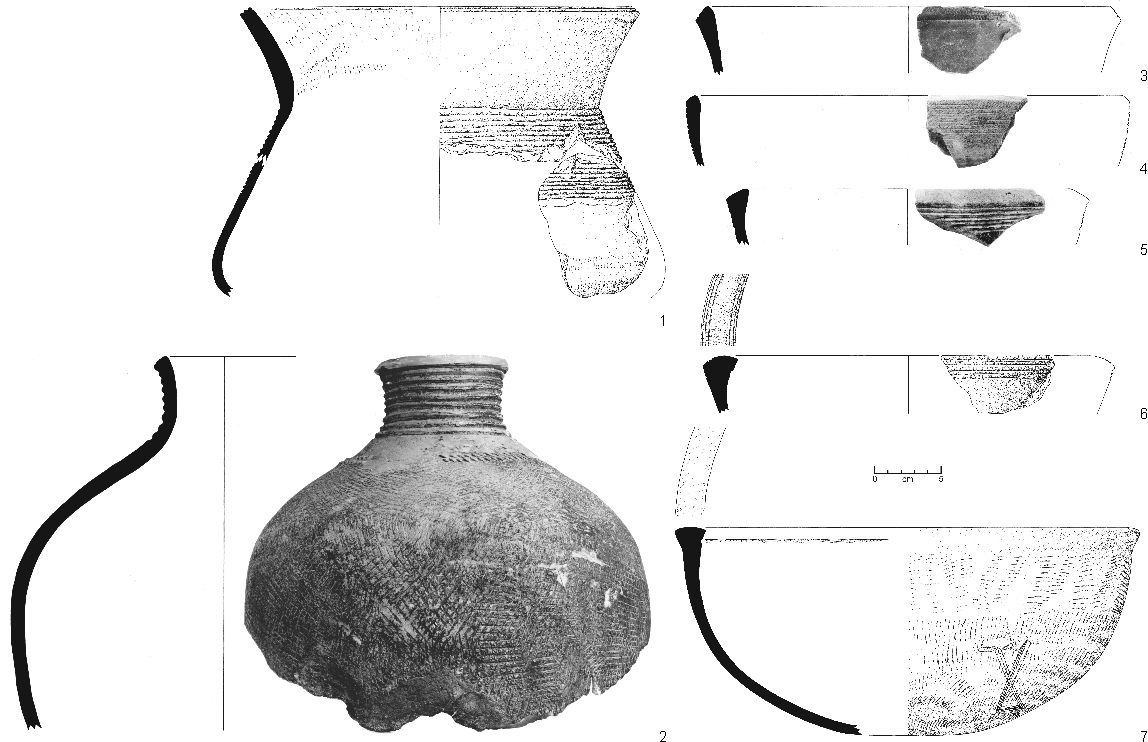
\includegraphics[width=\textwidth]{fig/BOT-Typen.pdf}
	\caption{Botendo-Gruppe: Typvertreter.\\1:~Taf.~71.2; 2:~Taf.~2.2; 3:~Taf.~4.4; 4:~Taf.~3.14; 5:~Taf.~34.8; 6:~Taf.~32.15; 7:~Taf.~68.5.}\label{fig:BOT_Typverteter}
\end{figure*}

\subsubsection{Botendo-Gruppe}\label{sec:BOT-Gr}

Die mindestens Ende des 19.~Jh. n.~Chr. noch in Gebrauch befindliche und von \textsc{Wotzka} (1995: 157\,f.) als sub-rezent eingestufte Botendo-Keramik ließ sich an insgesamt 24 Fundstellen im südlichen Abschnitt des Arbeitsgebietes nachweisen, vornehmlich entlang der Unterläufe der Flüsse \mbox{Ubangi} und \mbox{Likwala}-\mbox{aux}-\mbox{Herbes} sowie dem 1987 befahrenen Abschnitt des Kongo (Abb.~\ref{fig:BOT_Verbreitung}). Mehr als zehn GE der Botendo-Gruppe finden sich an lediglich sechs Fundstellen: 24~GE stammen aus Boleko am unteren \mbox{Likwala}-\mbox{aux}-\mbox{Herbes} (Fpl.~285), 21~GE aus Bobusa (Fpl.~239) und 19~GE aus Sosolo (Fpl.~241) am \mbox{Sangha}, 18~GE aus Gombe (Fpl.~237) am Kongo und 17~GE aus Bobangi (Fpl.~189) sowie zwölf GE aus Boyoka am unteren \mbox{Ubangi}. Insgesamt wurden 198 individuell aufgenommene GE der Botendo-Gruppe zugewiesen und 120 weitere Stücke ausgezählt erfasst. Während sich vier GE des Botendo-Stils im 1987 in Boleko am unteren \mbox{Likwala}-\mbox{aux}-\mbox{Herbes} ausgegrabenen Grab BLK~87/1 (Kat.-Nr.~14) fanden, sind weitere 30 unter Vorbehalt der Botendo-Gruppe zuweisbare GE bei der Ausgrabung mehrerer Schichten innerhalb der Grabung BBS~87/2 in Bobusa am unteren \mbox{Sangha} erfasst worden (Kat.-Nr.7). Die übrigen Stücke, die 89\,\% aller Botendo-Keramik im Arbeitsgebiet ausmachen, wurden bei Surveys moderner Dorfflächen gefunden. Die Zuweisung zur Botendo-Gruppe war lediglich bei 39\,\% aller Stücke zweifelsfrei möglich, während 61\,\% nur unter Vorbehalt der Stilgruppe zugerechnet werden konnten.\footnote{Dieser Umstand ist eine Folge der starken Fragmentierung jener Stücke aus den Oberflächensurveys; 62\,\% aller Stücke sind kleiner als 70\,$\times$\,70\,mm. Des Weiteren besteht das im Arbeitsgebiet erschlossene Inventar des Botendo-Stils zu knapp 30\,\% aus Wandungsscherben, die eine spärliche Verzierung aus horizontalen Rillen (Tab.~\ref{tab:Verzierungselemente}: 02.1) und flächigem \textit{banfwa-nfwa} (Tab.~\ref{tab:Verzierungselemente}: 08) aufweisen. Stücke mit diesen Merkmalen lassen sich kaum von Vertretern der Ebambe-Gruppe unterscheiden (Kap.~\ref{sec:EBA-Gr}).}

\paragraph{Technologische Merkmale}\hspace{-.5em}|\hspace{.5em}%
Die Keramik der Botendo-Gruppe aus dem nordwestlichen Kongobecken zeichnet sich, wie alle auch aus dem angrenzenden Inneren Kongobecken bekannte Stilgruppen, durch das nahezu vollkommenden Fehlen nichtplastischer Partikel im Scherben aus. In der Folge setzt sich das Inventar fast ausnahmslos aus Vertretern der \textit{Fabrics} 1 (81\,\%) sowie 2 (8\,\%) zusammen. Die restlichen Anteile entfallen auf Stücke, die allesamt nur unter Vorbehalt als der Botendo-Gruppe zugehörig angesehen werden können, darunter 23 vornehmlich aus Bobusa (Fpl.~239) und Boleko (Fpl.~285) stammende GE mit Schamott-Magerung, die dem \textit{Fabric} 9 zuzuordnen sind. Mit Blick auf die Färbung der Stücke lässt sich festhalten, dass 61\,\% aller Stücke eine Färbung aufweisen, die auf die Nutzung weißbrennender Tone hindeutet, während Indizien für die Nutzung rotbrennender Tone nur bei 9\,\% der Stücke beobachtet werden konnten. 

\paragraph{Formen}\hspace{-.5em}|\hspace{.5em}%
Bei 52~GE der Botendo-Gruppe kann die Gefäßform zweifelsfrei angesprochen werden. Bei 99 GE ist eine Ansprache nur unter Vorbehalt möglich. Die erfassten Inventare weisen ein 18 Typen umfassendes, heterogenes Spektrum an Gefäßformen auf. Kennzeichnend sind vor allem schalenförmige Gefäße mit konvexer Wandung vom Typ I3 (36\,\%; Abb.~\ref{fig:BOT_Typverteter}.7) sowie schalenförmige Gefäße mit abknickender Wandung und leicht ausbiegendem Oberteil vom Typ G6 (32\,\%). Bereits deutlich seltener lassen sich Gefäße mit geschweifter Wandung vom Typ E1 (E1; 10\,\%; Abb.~\ref{fig:BOT_Typverteter}.1) nachweisen. Unter ausschließlicher Berücksichtigung der Grundform stellen schalenförmige Gefäße mit konvexer Wandung (Typ~I) mit einem Gesamtanteil von 38\,\% sowie solche mit abknickender Wandung (Typ G) mit einem Anteil von 34\,\% die bestimmenden Gefäßformen dar. Gefäße mit geschweifter Wandung (Typ~E) machen zusammen 13\,\% aus, während die übrigen Grundformen -- wie flaschenförmige Gefäße (Abb.~\ref{fig:BOT_Typverteter}.2) -- lediglich als Einzelfunde beobachtet werden konnten. Die Schalen weisen Durchmesser zwischen 11--45\,cm und Höhen von 6--16\,cm auf. Das Verhältnis zwischen maximalem Durchmesser, im Fall der Schalen entspricht dieser der Weite der Mündung, und Höhe liegt im Mittel bei etwa 2:1. Die Schalen sind regelhaft etwa doppelt so breit wie hoch.\footnote{Aufgrund der starken Fragmentierung konnte lediglich bei 18 GE die Höhe der Mündung und somit das Verhältnis zum maximalen Durchmesser ermittelt werden.} Das Spektrum der Randformen kann anhand von 169~GE beschrieben werden.\footnote{Gerade aufsteigende Randformen (A) machen insgesamt 57\,\% aller beobachten Ränder aus. Knapp 37\,\% konnten als ausbiegende Randformen (B) angesprochen werden, während einbiegende Varianten (C) lediglich 6\,\% ausmachen.} Es ist ähnlich zahlreich an individuellen Typen, wie dies bei den Gefäßformen der Fall ist und wird vornehmlich von gerade aufsteigenden, im Profil dreieckig verdickten und gerade oder schräg nach außen abgestrichenen Rändern des Typs A4.3 bestimmt (45\,\%; Abb.~\ref{fig:BOT_Typverteter}.3--7). Ausbiegende, im Profil dreieckig verdickte Ränder mit schräg abgestricher Randlippe vom Typ B1.3 machen 9\,\% der beobachteten Ränder aus. Selten finden sich einfach ausbiegende (B1; 12\,\%) oder parallel aufsteigende Ränder (A1; 11\,\%). Weitere Variationen paralleler oder ausbiegender Ränder kommen in einzelnen Ausprägungen vor. Bei zwölf GE ist eine Ansprache der Bodenform möglich. Neun GE zeigen einen runden Boden vom Typ B1 (75\,\%, Abb.~\ref{fig:BOT_Typverteter}.7; Taf.~34.5, 68.2). Die übrigen drei GE, die lediglich unter Vorbehalt der Botendo-Gruppe zugerechnet werden können, weisen einen abgesetzten flachen Boden (B11; Taf.~69.1), einen flachen Boden mit deutlich einziehender Unterseite (B12; Taf.~1.4) und einen Standringboden (B13) auf.

\begin{figure*}[p]
	\centering
	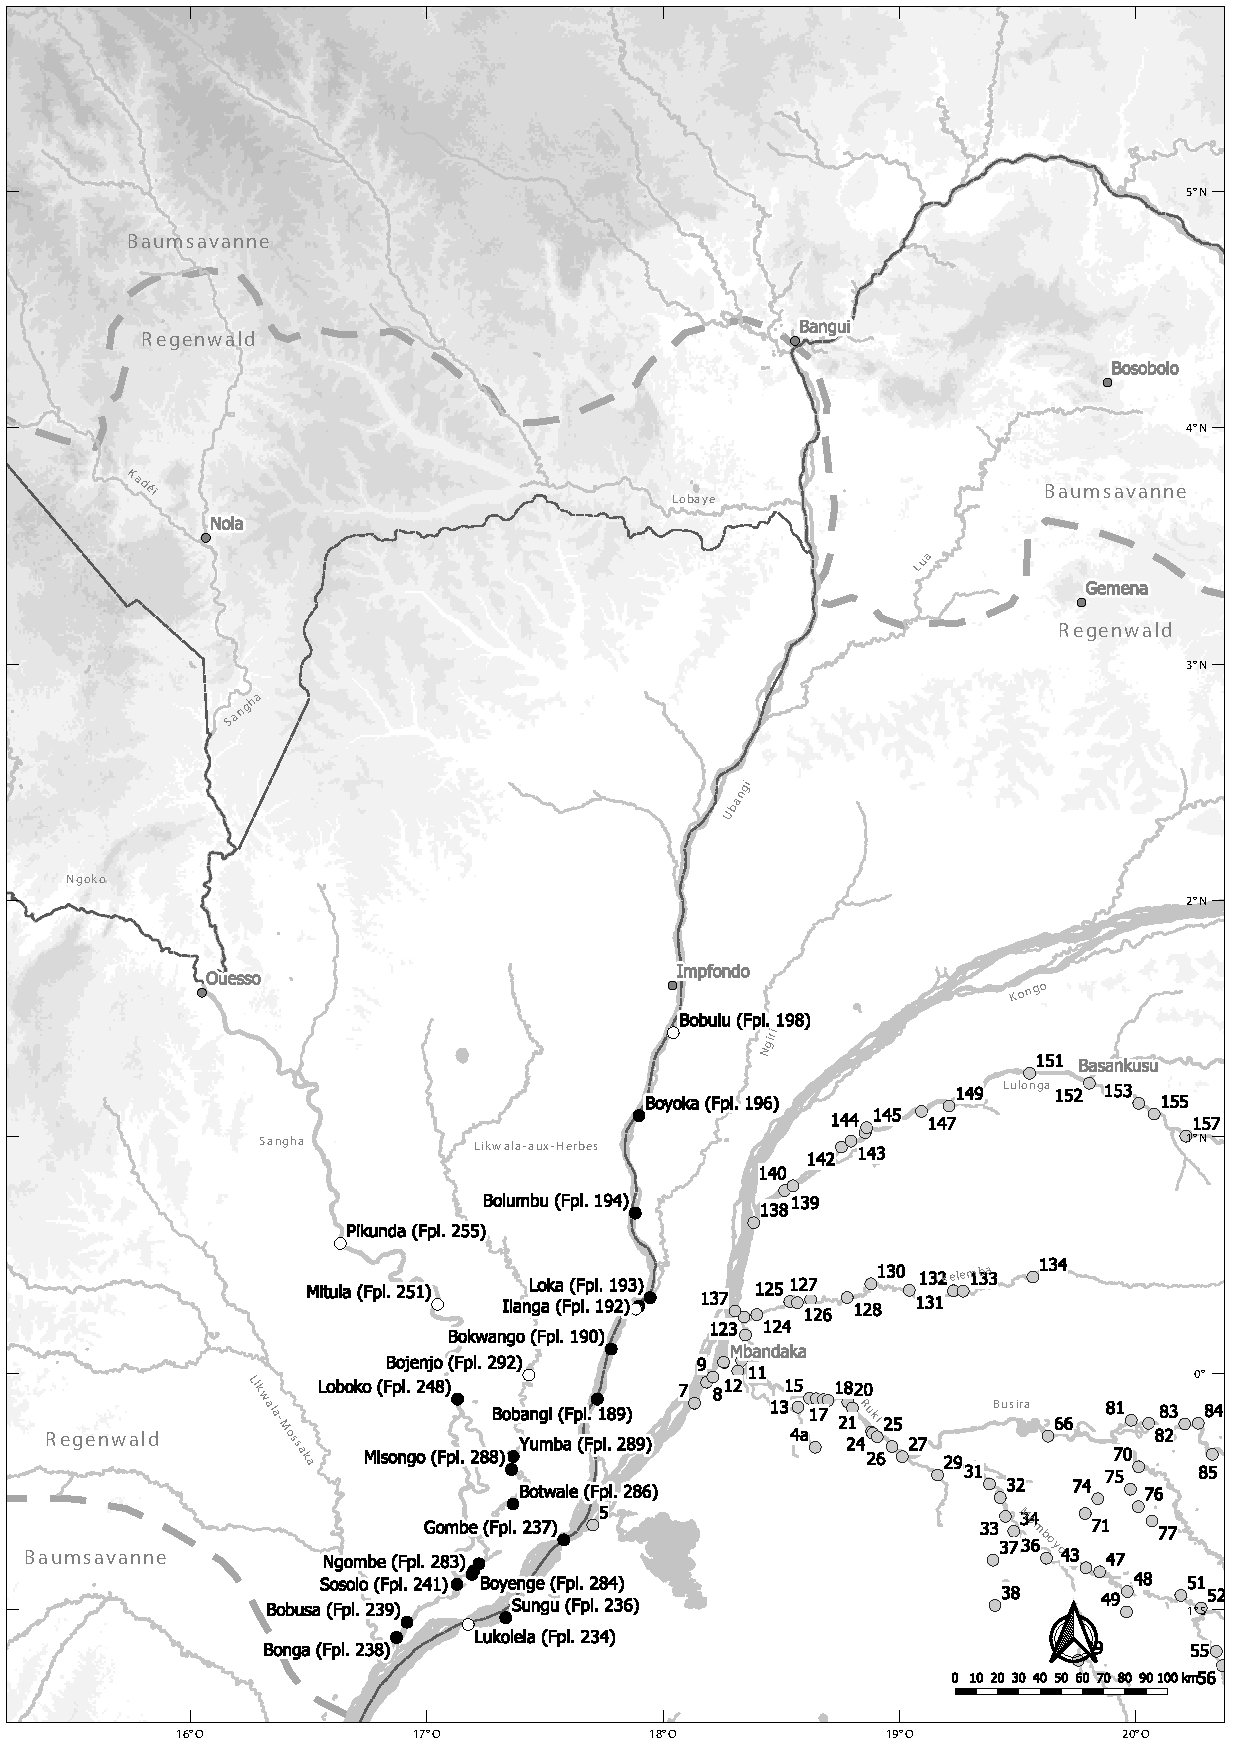
\includegraphics[width=\textwidth]{fig/BOT_Verbreitung.pdf}
	\caption{Botendo-Gruppe: Verbreitung im Arbeitsgebiet sowie im Inneren Kongobecken \parencite[grau; nach][572--573 Karte 16]{Wotzka.1995}.}
	\label{fig:BOT_Verbreitung}
\end{figure*}

\paragraph{Verzierungen}\hspace{-.5em}|\hspace{.5em}%
Die Verzierungen der Botendo-Keramik beschränken sich fast ausschließlich auf zwei Verzierungselemente: flächiges \textit{banfwa-nfwa}, dass regelhaft innen am Rand sowie auf dem Bauch der Gefäße zu beobachten ist (Abb.~\ref{fig:BOT_Typverteter}.1,7) und 45\,\% aller aufgenommenen Verzierungselemente ausmacht, sowie horizontale Rillen (Tab.~\ref{tab:Verzierungselemente}: 02.1), die sich vornehmlich innen wie außen im Randbereich finden (Abb.~\ref{fig:BOT_Typverteter}.2,5) und 38\,\% aller Verzierungselemente widerspiegeln. Bänder und Reihen bildende Eindrücke (Tab.~\ref{tab:Verzierungselemente}: 04) machen zusammen knapp 10\,\% aller Verzierungselemente aus. Generell zeigt die Botendo-Keramik im nordwestlichen, wie auch jene im Inneren Kongobecken (ebd. 154--156) eine etwas reichhaltigere Ornamentik als die rezenten Keramikgruppen Epena (Kap.~\ref{sec:EPE-Gr}) beziehungsweise Ikenge \parencite{Eggert.1980c}. Insgesamt sind 77\,\% aller der Botendo-Gruppe zugeordneten GE überhaupt verziert und über 75\,\% aller Stücke weisen lediglich zwei oder weniger Verzierungselemente auf. Die am häufigsten verzierten Bereiche der Botendo-Keramik sind die Innenseiten der Ränder, an denen sich 33\,\% aller Verzierungselemente finden sowie die Außenseiten der Ränder, die mit 36\,\% aller aufgenommenen Verzierungen sogar noch etwas häufiger verziert sind. Grundsätzlich kann festgehalten werden, dass Innen- und Außenseite der Ränder bei GE der Botendo-Gruppe regelhaft mit \textit{banfwa-nfwa} sowie horizontalen Rillen verziert sind. Mit etwa 17\,\% aller Verzierungselemente sind die Bauchbereiche bereits deutlich seltener verziert; wenn, dann fast ausschließlich mit flächigem \textit{banfwa-nfwa}.


\paragraph{Datierung}\hspace{-.5em}|\hspace{.5em}%
Eigenständige Datierungsansätze für die chronologische Ansprache der Botendo-Keramik ergaben sich durch die Funde aus dem nordwestlichen Kongobecken nur bedingt. Einzig in einem (sub)rezenten Grab in Boleko am Likwala-aux-Herbes (Fpl.~285; Kat.-Nr.~14) wurden fünf dem Botendo-Stil zuweisbare GE entdeckt. Diese Beobachtung lässt sich der von \textcite[156--158]{Wotzka.1995} erarbeiteten Datierung des Botendo-Stils, die sich aus drei unabhängigen Quellen speist, hinzusetzen.\footnote{Der Datierungsansatz für den Botendo-Stil setzt sich bislang aus den folgenden drei Quellen zusammen: Vertreter der Botendo-Gruppe finden sich in der Veröffentlichung von ethnografischen Keramikbeständen des damaligen \textit{Musée du Congo} (heute \textit{Musée royal du l'Afrique centrale}) in Tervuren bei Brüssel \parencites[155--157 Taf.~12]{Coart.1907}[157]{Wotzka.1995}. Daraus folgert \textsc{Wotzka} (ebd.), dass die Botendo-Keramik zumindest in den letzten Jahrzehnten des 19.~Jh.~n.~Chr. noch zu den \enquote{Produkten der zeitgenössischen traditionellen Töpferei} gehörte. Den zweiten Datierungsansatz liefert der Befund aus der 1915 aufgelassenen Dorfwüstung von Nkile am Ruki (Fpl.~17), in der Keramik der Botendo-Gruppe die jüngste archäologisch erfasste Besiedlungsphase bildet (ebd. 157\,f.). Eine 1895 durchgeführte Zählung der Dörfer am Ruki führt die Siedlung als noch bewohnt auf, während 1977/78 im benachbarten Bokuma (Fpl.~18) von M.~K.~H. Eggert aufgenommene orale Tradition eine Auflassung der Siedlung um 1915 andeutet (ebd. 315). Das dritte Datierungsindiz bilden zwei Radiokohlenstoffdatierungen aus dem Befund NKI~2 in Nkile, die beide mit Keramik der Botendo-Gruppe assoziiert sind. Während eine Probe ein rezentes Probenalter erbrachte, datiert die Zweite in das 17.--20.~Jh. n.~Chr. (ebd. 158 Tab.~70).} Gegenwärtig kann das Bestehen des Botendo-Stils auf das 18. bis frühe 20.~Jh. n.~Chr. eingegrenzt werden.

\paragraph{Verbreitung}\hspace{-.5em}|\hspace{.5em}%
Keramik der Botendo-Gruppe findet sich im südlichen Abschnitt des Arbeitsgebietes, vornehmlich entlang des unteren \mbox{Ubangi} bis nach Boyoka (Fpl.~196; Abb.~\ref{fig:BOT_Verbreitung}). Weitere GE des Botendo-Stils wurden zwischen Yumba (Fpl.~289) bis zur Einmündung des \mbox{Likwala}-\mbox{aux}-\mbox{Herbes} in den \mbox{Sangha} bei Sosolo (Fpl.~242) gefunden. Nördlich der Einmündung des \mbox{Likwala}-\mbox{aux}-\mbox{Herbes} fand sich entlang des unteren \mbox{Sangha} vergleichsweise wenig Botendo-Keramik. Lediglich in Loboko (Fpl.~248) konnte Botendo-Keramik sicher nachgewiesen werden. Der kurze Abschnitt am unteren \mbox{Sangha} zwischen der Einmündung des \mbox{Likwala}-\mbox{aux}-\mbox{Herbes} sowie der Einmündung des \mbox{Sangha} in den Kongo zählt ebenso zum Verbreitungsgebiet wie der 1987 prospektierte Abschnitt des Kongo zwischen der Mündung des \mbox{Sangha} im Süden und des \mbox{Ubangi} im Norden. Stromauf von Boyoka am \mbox{Ubangi} (Fpl.~196) und Loboko am \mbox{Sangha} (Fpl.~248) fanden sich lediglich wenige und nur unter Vorbehalt der Botendo-Gruppe zuweisbare Stücke (Abb.~\ref{fig:BOT_Verbreitung}). Das Verbreitungsgebiet der Botendo-Keramik im Inneren Kongobecken umfasst vor allem die Flussgebiete des Ruki-Momboyo-Luilaka, des Busira und Ikelemba sowie des Lulonga und unteren Maringa (ebd. 158, 572--573 Karte 16). Im östlichen Abschnitt des von \textsc{Wotzka} (ebd. 572--573 Karte 16) untersuchten Inneren Kongobeckens, entlang des Lopori, des oberen Maringa sowie des gesamten Tshuapa fanden sich keine Vertreter der Botendo-Gruppe. Zusammengenommen ist der Botendo-Stil in einem etwa 350\,km (Nord--Süd) $\times$ 450\,km (Ost--West) großen Gebiet verbreitet.\footnote{Die westlichste Fundstelle dieses kombinierten Verbreitungsgebietes bildet Bonga an der Mündung des \mbox{Sangha} (Fpl.~238), während der östlichste Fundpunkt in Baulu am Maringa liegt (Fpl.~162). Die nördlichste Fundstelle ist Bonkita am Lulonga (Fpl.~151) und die südlichste Bekongo am Luilaka (Fpl.~60).}